
\documentclass[lineno]{jfm}

\usepackage{graphicx}
%\usepackage{epstopdf,epsfig}
\usepackage{newtxtext}
\usepackage{newtxmath}
\usepackage{natbib}
\usepackage{hyperref}
\usepackage{mathtools}
\usepackage{commath}




\hypersetup{
    colorlinks = true,
    urlcolor   = blue,
    citecolor  = black,
}
\newtheorem{lemma}{Lemma}
\newtheorem{corollary}{Corollary}
\newcommand{\RomanNumeralCaps}[1]
\linenumbers


% {\MakeUppercase{\romannumeral #1}}

%\title{Two-Dimensional Vesicles Under External Flow via Integral Equation Method}
\title{Modeling Two-Dimensional Vesicle Hydrodynamics with Hydrophobic Attraction Potential Simulations}
%\author{Alan N. Jones\aff{1}
%  \corresp{\email{JFMEditorial@cambridge.org}},
%  H.-C. Smith\aff{1}
% \and J.Q. Long\aff{2}}
%
%\affiliation{\aff{1}STM Journals, Cambridge University Press, The Printing House, Shaftesbury Road, Cambridge CB2 8BS, UK
%\aff{2}DAMTP, Centre for Mathematical Sciences, Wilberforce Road, Cambridge CB3 0WA, UK}


\author{
Szu-Pei Fu\aff{1},
Bryan Quaife\aff{2},
Rolf Ryham\aff{1}, \and
Yuan-Nan Young\aff{3}
}
 \affiliation{
\aff{1} Department of Mathematics, \\Fordham University, Bronx, New York 10458, USA
\aff{2}Department of Scientific Computing, \\Florida State University, Tallahassee, Florida 32306, USA
\aff{3}Department of Mathematical Sciences, New Jersey Institute of Technology,\\ Newark, New Jersey 07102, USA
 }





\begin{document}
\maketitle

\begin{abstract}
In this work, we study the dynamics of many-body systems immersed in a viscous fluid with a specified interparticle force. In particular, we apply a hydrophobic attraction potential (HAP) using a Janus type granular system to model lipid bilayer membranes. Coupling with an efficient integral equation method for rigid bodies in Stokes flow and an previous developed HAP solver, the deformations of a two-dimensional vesicle such as tank-treading motion and membrane ruptures can be observed under different values of the shear rate. Moreover, an efficient integral equation method is adopted for solving the screened Laplace equation and the mobility problem where it can accurately calculate hydrophobic and hydrodynamic interactions between near touched boundaries.
\end{abstract}


\begin{keywords}
Authors should not enter keywords on the manuscript, as these must be chosen by the author during the online submission process and will then be added during the typesetting process (see \href{https://www.cambridge.org/core/journals/journal-of-fluid-mechanics/information/list-of-keywords}{Keyword PDF} for the full list).  Other classifications will be added at the same time.
\end{keywords}

{\bf MSC Codes }  {\it(Optional)} Please enter your MSC Codes here



\section{\label{intro}Introduction}







\section{Governing  Equations}
\subsection{Hydrophobic Attraction Potential (HAP)}


The Hydrophobic attraction potential (HAP) is given by
\begin{equation}
\label{eq:main}
\Phi(\Omega,f) = \gamma  \min_{u \in \mathcal{A}}
 I[u]  = \int_{\Omega} \rho |\nabla u|^2 + \rho^{-1} u^2 \,dx,
\end{equation}
%
where $\gamma$ the interfacial tension, $\rho$ the screened length, and this domain functional describes the energy associated with hydrophobic surfaces~\cite{Fu20}. From the first domain variation of HAP, we obtain a hydrophobic stress tensor which is given as follows, 

\begin{equation}
\label{eq:stress}
\mathbf{T}
= \gamma\rho^{-1}u^2 \mathbf{I} + 2\rho\gamma (\tfrac{1}{2}|\nabla u|^2 \mathbf{I} - \nabla u\otimes \nabla u).
\end{equation}
%
The integration over boundaries gives force and torque due to the hydrophobic attraction and they are given by 

\begin{equation}
\int_{\Gamma_i} {\bf T}\cdot \nu_i dS ,\quad \int_{\Gamma_i} ({\bf x}-{\bf a}_i)\times ({\bf T}\cdot \nu_i) dS,
\end{equation}
%
where ${\bf x}$ are points on the boundary $\Gamma_i$, ${\bf a}_i$ is the $i^{th}$ particle center, and $\nu_i$ is the outward normal to the $i^{th}$ particle.


%\begin{equation}
%        \label{SL}
%\begin{cases}
% -\rho^2 \Delta u + u =0 & \text{ in } \Omega,\\
%  u(x) = f(x)  &\text{ on }\Sigma, \\
%   u(x) \to 0, &\text{ as } x \to \infty.
%\end{cases}
%\end{equation}

\subsection{Nondimensionalizations}



For a two-dimensional vesicle, we denote a constant initial radius $R_0$ and 
the dimensionless shear rate is
\begin{equation}
\chi = \dot\gamma \cdot\frac{\mu R_0^2}{\kappa},
\end{equation}
%
where $\dot\gamma$ the shear rate, $\kappa$ the bending rigidity, and $\mu$ the fluid viscosity~\cite{Finken08}.


%This paper is organized as follows. Chapter 2 introduces the mobility problem..... The integral equation method for solving $N_b$-body system with details of .... are included in Chapter 3. We provide numerical results of vesicle simulations in Chapter 4. Finally, we conclude the work and briefly give the picture of our future work.


\subsection{\label{mobility}Mobility Problem}

The governing equation of $N_b$-body bodies suspended in the domain $\Sigma$ is
 
\begin{gather}
	-\Delta {\bf u} + \mu\nabla p = 0 \qquad \text{in }\Sigma\\
	\nabla\cdot {\bf u}=0 \qquad \text{in }\Sigma\\
	{\bf u}({\bf x}) \to {\bf u}_\infty \quad \text{as}\quad |{\bf x}|\to \infty
\end{gather}
%
where ${\bf u}$ is the velocity, $p$ is the pressure, and ${\bf u}_\infty$ is the background flow. 
%
%\begin{gather}
%\int_{\Gamma_i}(\sigma_{hyd}+\sigma_\infty)\cdot {\bf n} ds = -{\bf F}_i \\
%	\int_{\Gamma_i}(\sigma_{hyd}+\sigma_\infty)\times({\bf x}-{\bf a}_i)\cdot {\bf n} ds =-\tau_i\\
%\end{gather}
%
The mobility problem for $N_b$-body system in a Stokes flow leads to a second-kind boundary integral equations (BIE) with a density function $\eta({\bf x}$ that is given by \cite{Lukas19}
\begin{equation}
\label{mobility}
\begin{aligned}
{\bf v}_i + &\omega_i\times({\bf x}-{\bf a}_i)\\
 =& -\frac12\eta({\bf x}) + D[\eta]({\bf x}) \\
&+ \sum_{i=1}^N\big({\bf S}({\bf x}, {\bf a}_i){\bf F}_i+ {\bf R}({\bf x}, {\bf a}_i)t_i\big)+{\bf u}_\infty, \quad {\bf x}\in\Gamma \\
\end{aligned}
\end{equation}
%
with two constraints 
%
\begin{center}
\begin{equation}
\label{mobility2}
\int_{\partial \Gamma_i}\eta\cdot \nu ds = {\bf 0},
\end{equation}
\end{center}
%
\begin{center}
\begin{equation}
\label{mobility3}
\int_{\partial \Gamma_i}\eta\times({\bf x}-{\bf a}_i)\cdot \nu ds ={\bf 0},
\end{equation}
\end{center}
%
where the two-dimensional Stokeslet and the Rotlet are
%
\begin{gather}
{\bf S}({\bf x}, {\bf a}) = \frac{1}{4\pi}\left(-\log(|({\bf x}-{\bf a})|){\bf I}+\frac{({\bf x}-{\bf a})\otimes({\bf x}-{\bf a})}{|({\bf x}-{\bf a})|^2}\right) \\ 
{\bf R}({\bf x},{\bf a})=\frac{({\bf x}-{\bf a})^\perp}{4\pi|({\bf x}-{\bf a})|^2}.
\end{gather}
%
%Here ${\bf r}={\bf x}-{\bf a}$ and $\rho=|{\bf r}|$.
${\bf F}_i$ and $t_i$ are particle force and torque calculated from action of hydrophobic attractions. From equations~\eqref{mobility}--\eqref{mobility3}, we have translational velocity ${\bf v}_i$, angular velocity $\omega_i$, and density function $\eta$ as unknowns.
This system of equations is then solvable with the use of an iterative method such as GMRES or conjugate gradient iterations.

\subsection{Short Range Repulsion}

At each time step, we examine the nearest grid points between each pair of body  boundaries. Within a specified distance $d$, we introduce a short range repulsive potential as follows

\begin{equation}
\Phi_{repul} = 1- \sin\left(\frac{\pi}{2} d\right).
\end{equation}

Here we would like to make a remark about the time marching scheme. From the mobility problem, we obtain velocity and torque profiles of an $N_b$-body system. A second order Adam-Bashforth scheme is used for updating the dynamics but body collisions may occur during the simulation while a relatively large time step is chosen. We therefore impose a short range repulsion that it will be turned on when the distance between two boundary points on different bodies are within one characteristic length.


%%%


\section{\label{IEM}Integral Equation Method}



%%%


\section{\label{validation}Model Validation}

\subsection{Jeffery Orbit}


The preliminary test of the proposed model using the integral equation method is the numerical validation in Jeffery orbits of single ellipsoidal particle under a shear flow $\dot x = \dot\gamma y$ where $\dot\gamma$ is the shear rate. An ellipsoidal particle is initially placed with its center of mass fixed at the origin and the angle between the major axis and the $y$-axis is denoted as $\chi = 0^\circ$. Based on the theoretical Jeffery orbits with respect to the target angle $\chi(t)$, 

\begin{equation}
\chi(t) = \tan^{-1}\left(\frac{a}{b}\tan \left(\frac{ab \dot\gamma t}{a^2+b^2}\right)\right),
\end{equation}
%
where $a$, $b$ are semi-major and semi-minor axes, and the test aspect ratio of the particle is $2$. Figure~\ref{figure1} shows that the proposed integral equation method has a perfect agreement with the theoretical result from Jeffery orbits.


\begin{figure}
\centering
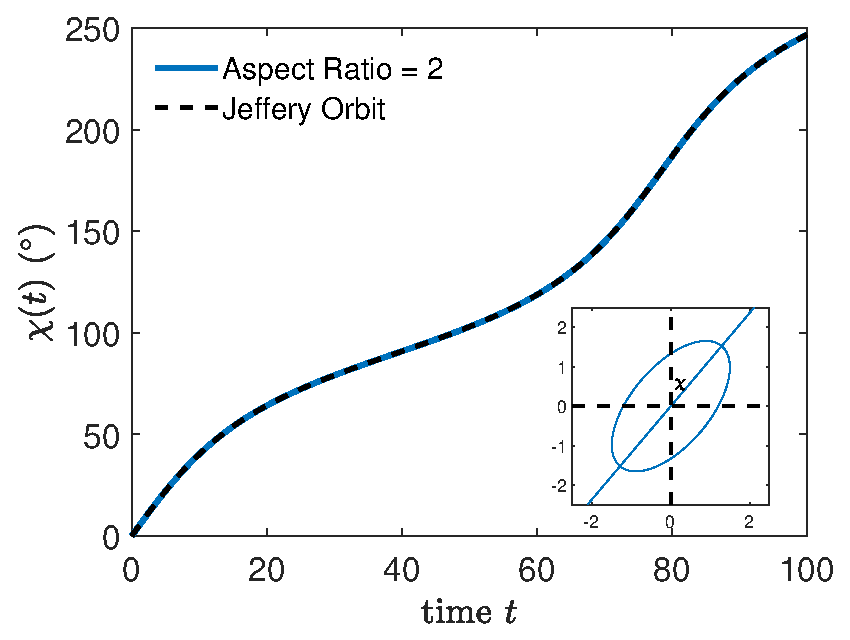
\includegraphics[width=0.4\textwidth]{JefferyOrbit.eps}
  \caption{Comparison of the target angle $\chi(t)$ versus time $t$ between the theoretical Jeffery orbit with $\dot\gamma=0.1$ and the result from the integral equation method. The schematic of the simulation setup is shown in the inset of the figure.
  }
    \label{figure1}
\end{figure}

\subsection{Self-Assembly and Relaxtion}

To study the deformation of a closed bilayer structure under a shear flow using the proposed algorithm, 
we adopt a widely tested numerical simulation in both continuum and molecular dynamics models, single vesicle under a shear flow. The well known results indicate that the vesicle does tank-treading when there is no viscosity contrast in both inside and outside of the structure.
Given a set of various shear rates, with no viscosity difference between internal and external fluids, 
the vesicle-like granular structure is initially placed in a quiescent flow for obtaining an equilibrium shape.


For the target bilayer, a circular initial shape is chosen to perform the relaxation run. This vesicle-like 
structure consists of $N=58$ disks with radius $r=0.5$ and the starting diameter for the vesicle is about 
$8.5$ length units.
The starting center of mass position of the vesicle is pinned at the origin and we track particle velocities 
to determine the initial configuration for later use such as single and multiple vesicle simulations. This will prevent some numerical instability issues when the minimum of the total energy is not achieved. For instance, the dynamics of the bilayer under a shear flow may reach different outcomes.
Figure~\ref{figure2} shows that the magnitudes of mean velocity components ${\bf v}=\{v_x,v_y\}$ decrease exponentially with an approximation decaying rate $\sim0.005$. In the same figure, the variation of mean particle orientation $\theta$ also decreases as expected. The time step size 
$\Delta t=0.2$ is used for all simulations including the relaxation run.

\begin{figure}
\centering
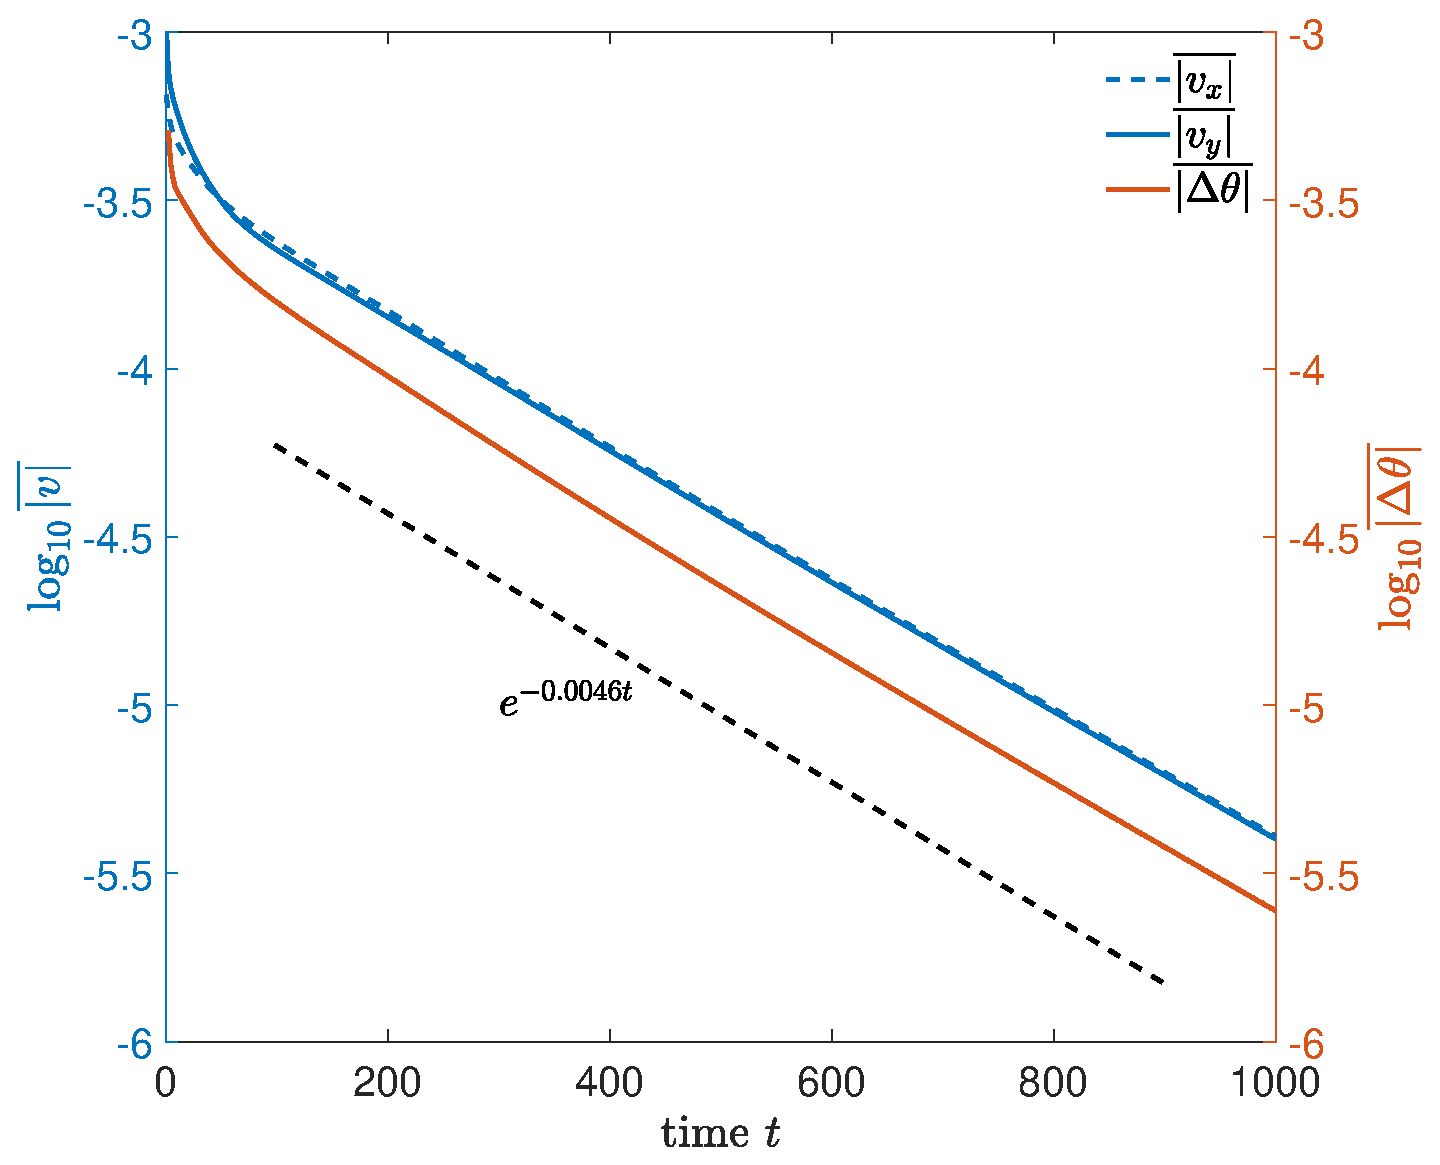
\includegraphics[height=2in]{relax.eps}
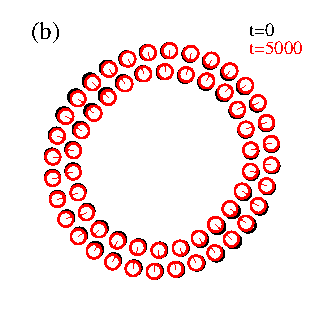
\includegraphics[height=2in]{relax2.eps}
  \caption{Vesicle relaxes under a quiescent flow. The blue dashed curve and the solid curve are mean magnitudes of the particle velocities in $x$ and $y$ directions, respectively. The red curve shows the decreasing trend of the mean magnitude of particle orientation change. The black dashed line shows the reference of how all magnitudes decay.
  }
    \label{figure2}
\end{figure}




%%%


\section{\label{results}Numerical Results}

\subsection{Tank-Treading Vesicles}

\subsubsection{Vesicle in a Shear Flow}

The snapshots of the simulation for single vesicle in a shear flow are shown in Figure~\ref{figure3}.
Panel (a) shows the initial circular shape obtained from the relaxation run and the deformed 
configuration of the vesicle after a period of time ($t=4000$) is in panel (c). The color presented in the figure 
is the strength of the action due to the hydrophobic attraction. From weak to strong action field, the color
varies from blue to red.
To demonstrate the tank-treading behavior of the vesicle, panels (b) and (d) provide the streamlines of the 
fluid velocity over the whole computational domain when the shear flow passes through the vesicle. The tank-treading motion of the structure is then observed.

% needs to add more details about inclination angle, tank-treading frequency, repulsion, ...etc.


\begin{figure}
\centering
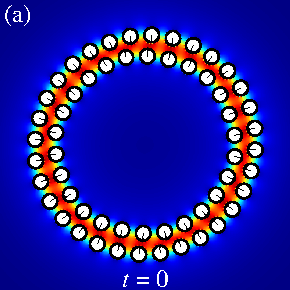
\includegraphics[width=0.3\textwidth]{N58_0.pdf}
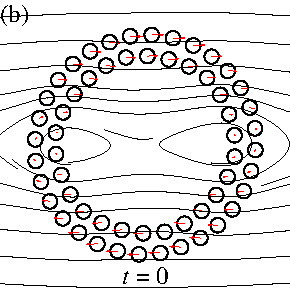
\includegraphics[width=0.3\textwidth]{N58_vel_0.pdf}\\
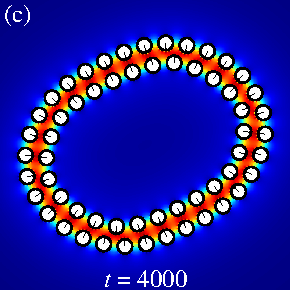
\includegraphics[width=0.3\textwidth]{N58_20000.pdf}
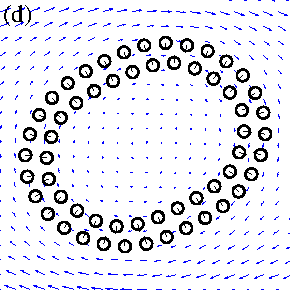
\includegraphics[width=0.3\textwidth]{N58_vel_20000.pdf}
  \caption{Vesicle under a shear flow where the shear rate $\dot\gamma=0.0025$: 
  (a) Initial configuration of 58-body vesicle; 
  (b) The fluid velocity plot with respect to the configuration in (a); Streamlines are plotted in the background
  as solid curves. Red arrows represent the particle velocities.
  (c) Deformed vesicle after $20000$ steps. The tank-treading motion occurs after reaching the state shown in panel (c).
  (d) The fluid velocity plot with respect to the configuration in (c);
  The background colors in panels (a) and (c) represent the strength of the hydrophobic attraction potential. The blue region shows no action and the red region with the bilayer gives the strongest action.
  }
    \label{figure3}
\end{figure}
%

In order to extract more physical properties of the proposed model, we track the total length of the bilayer structure and the reduced area over the time. Here the enclosed area and the length of the structure are calculated from the midplane. 
These results are shown in Figure~\ref{figure4} where we compare results from a set of shear rates $\dot\gamma=\{0.002,0.0025,0.003,0.0035\}$. 
The reduced area is given by $A^* = 4\pi A/L^2$ where $A$ is the vesicle area and $L$ is the arc length of the vesicle with respect to the midplane. Since the starting configuration is close to a circular shape, the reduced are decreases from a value very close to $1$. It is clear that a slower shear rate generates a higher reduced area and has a faster convergence. The small oscillations in all results are due to the granularity of the bilayer which tend to having a slightly non-smooth curve in simulations. Overall the total lengths of the bilayer have the same converging value in all test shear rates. Moreover, based on the 
numerical experiments, we observe that the reduce area converges relatively early when the shear rate is lower than $\dot\gamma=0.003$. 

An interesting phenomenon also rises up in the proposed setup where the inter-monolayer slip occurs 
between two leaflets. When a shear rate is large enough, take $\dot\gamma = 0.005$ as an example, 
Figure~\ref{figure5} shows the schematic of the test. A particle pair is initially marked and we then track the positions and layer velocities over the time. It is clear to see that the outer leaflet always has larger 
tangential velocity than the one from inner leaflet. This inter-leaflet sliding matches what has been seen
in articles in molecular dynamics simulations. %%% need some citations

\begin{figure}
\begin{center}
\hspace{-1cm}
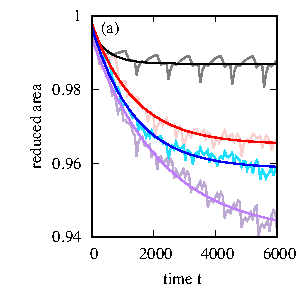
\includegraphics[height=2in]{ReducedArea.pdf}
\hspace{-1cm}
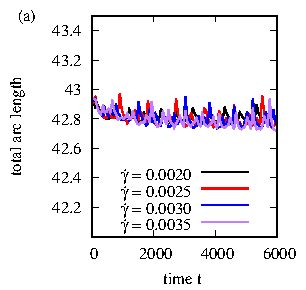
\includegraphics[height=2in]{ArcLength.pdf}
\hspace{-1cm}
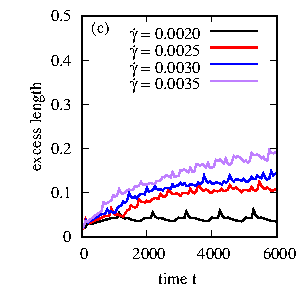
\includegraphics[height=2in]{ExcLength.pdf}
\end{center} 
  \caption{(a) Total arc lengths of the midplanes over time in different shear rates; (b) Reduced area transitions over time. 
A set of shear rates $\dot\gamma=\{0.002,0.0025,0.003,0.0035\}$ is used in simulations. 
A slower shear rate generates a faster convergence in the reduced area. 
  }
    \label{figure4}
\end{figure}





\begin{figure}
\begin{center}
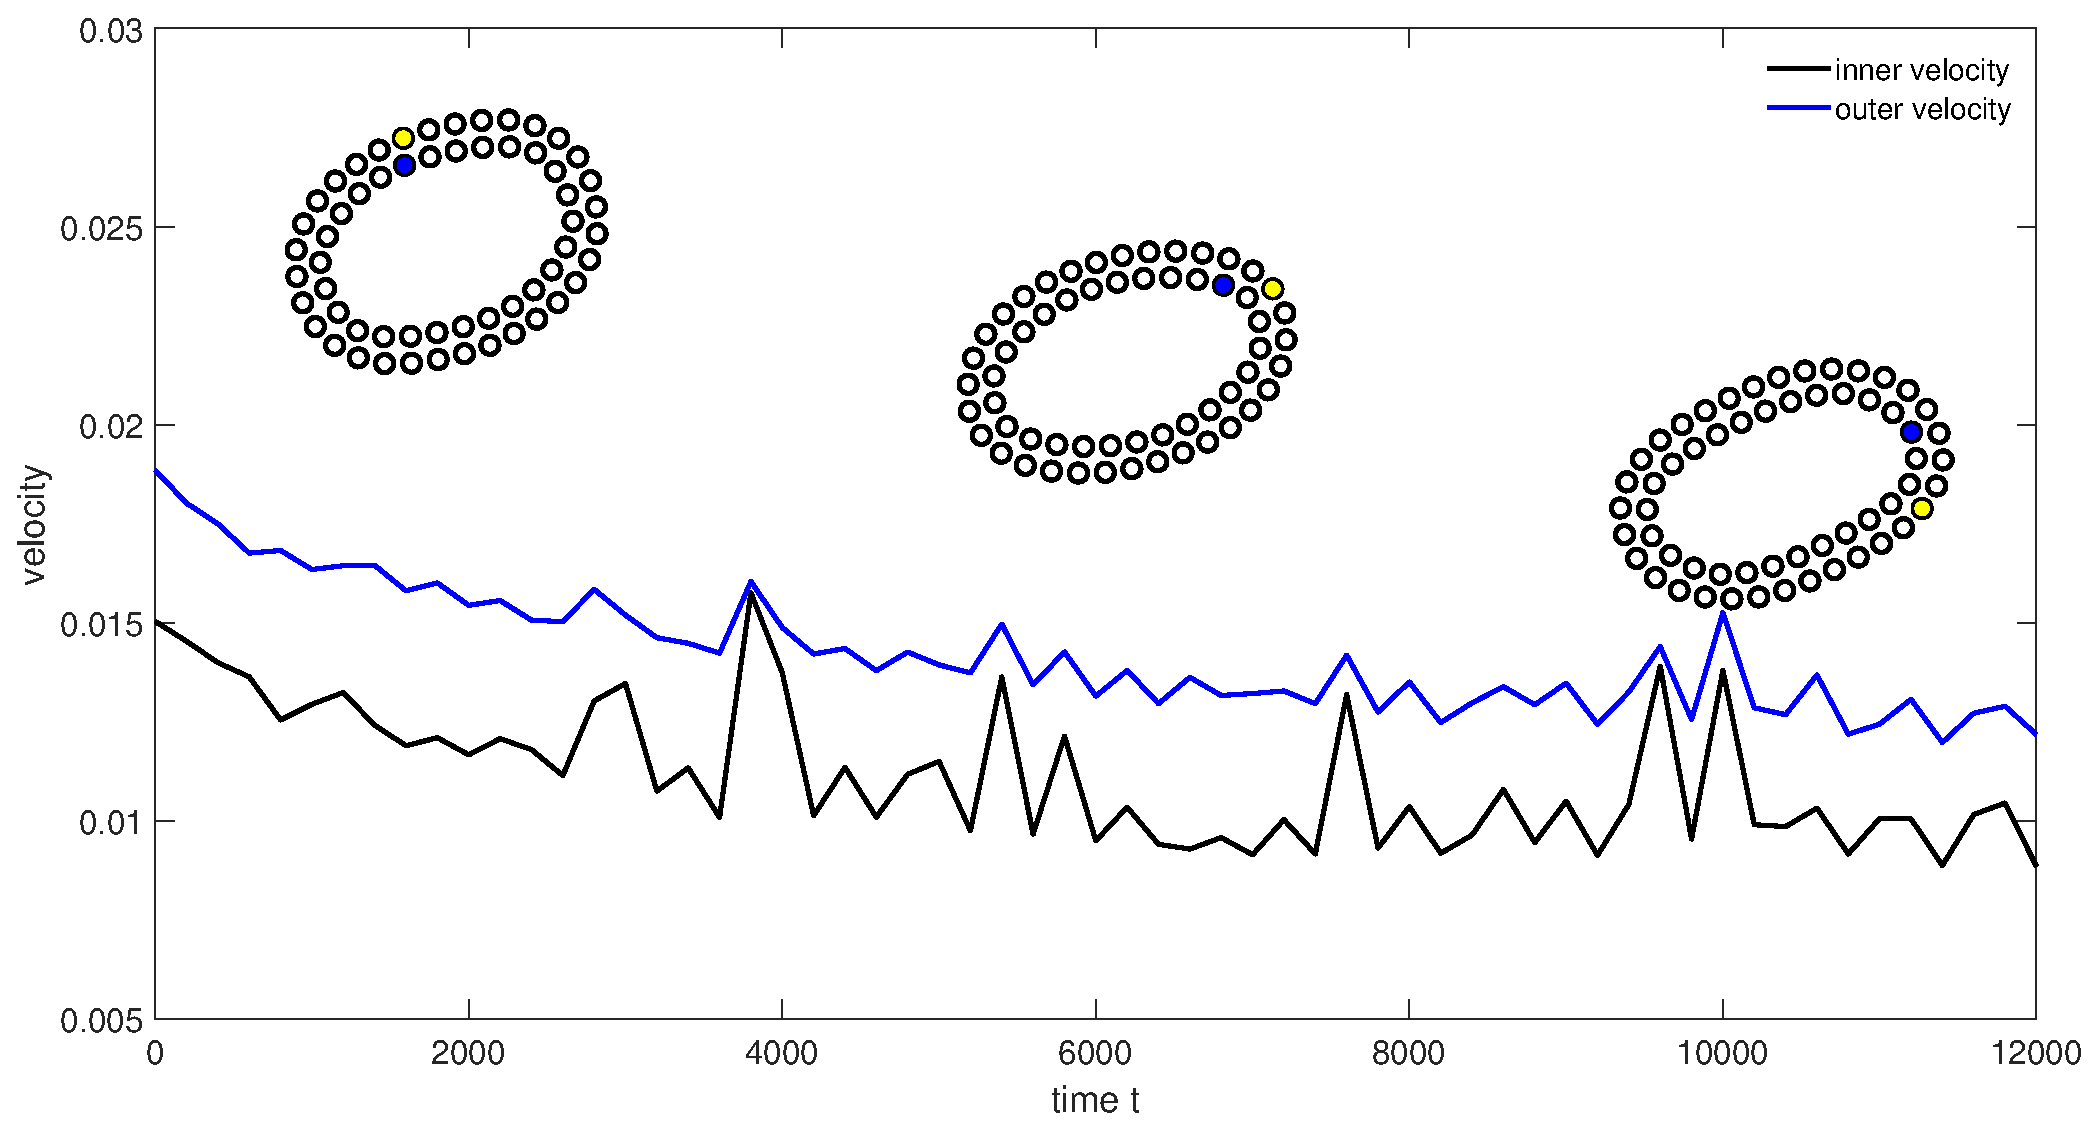
\includegraphics[width=0.8\textwidth]{Slip.eps}
\end{center} 
  \caption{For the shear rate $\dot\gamma=0.005$, the inter-monolayer slip is be observed. The curves in black and blue represent the tangential velocities of inner and outer leaflet, respectively. The configuration plots have two fixed particles marked and positioned with respect to the corresponding time $t$.
  }
    \label{figure5}
\end{figure}




\subsubsection{Vesicle in a Parabolic Flow}

The background flow for this set of simulations is given by

\begin{equation}
{\bf v}_\infty = v_{max}\left[ 1 - \left( \frac{y}{wR_0}\right)^2 \right]{\bf e}_x,
\end{equation}
%
where $v_{max}$ is the flow strength and $w$ controls the shape of the flow. $R_0$ is defined as the radius of the initial vesicle midplane. Figure~\ref{figure6} gives a final configuration for one specific case where the circular vesicle is initially placed above the $x$-axis.

\begin{figure}
\centering
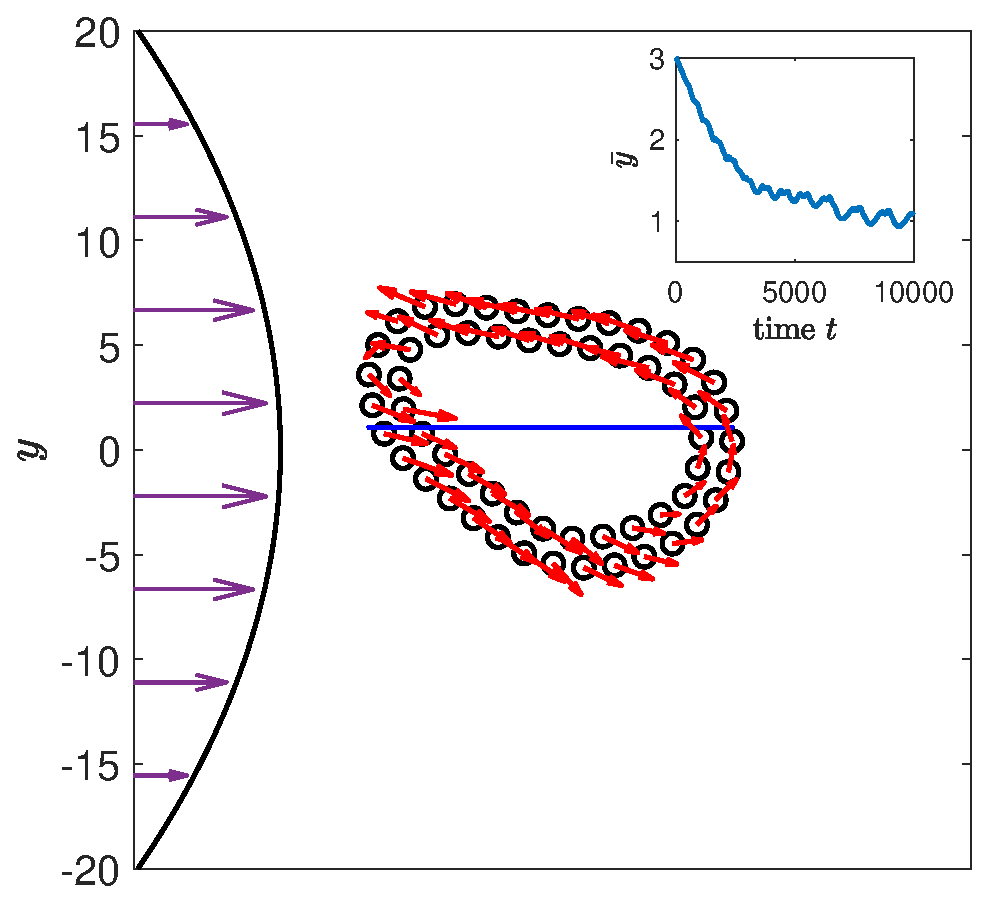
\includegraphics[width=0.5\textwidth]{parabolic.eps}
  \caption{Vesicle under a parabolic flow where the strength of the flow $v_{max}=8.0$ and the control parameter $w=10$. The configuration is the state when $t=10000$.
  }
    \label{figure6}
\end{figure}


\subsubsection{Membrane Ruptures}


With the choice of a large shear rate, a pore formation or a complete membrane rupture can be observed during simulations. Figure~\ref{figure7} shows a demonstration of a vesicle under a shear flow with shear rate $\dot\gamma=0.1$. An interesting phenomenon occurs in panels (c) and (d) where two separated bilayers move along the background shear flow symmetrically. Consequently, a periodic motion for bilayers may occur 
with the choices of shear rates. One can expect that these two layers will flow far apart from each other for much higher shear rates.



\begin{figure}
\centering
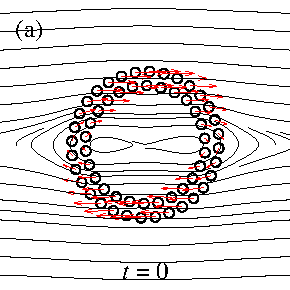
\includegraphics[height=1.2in]{N58_rupt_0.pdf}
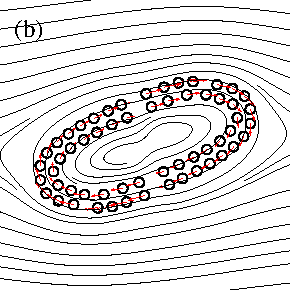
\includegraphics[height=1.2in]{N58_rupt_200.pdf}
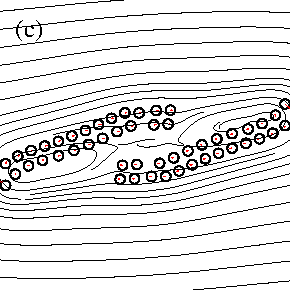
\includegraphics[height=1.2in]{N58_rupt_400.pdf}
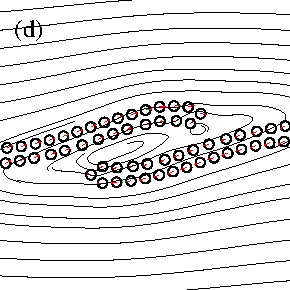
\includegraphics[height=1.2in]{N58_rupt_600.pdf}
  \caption{Membrane rupture occurs when the shear rate is beyond a certain threshold. Here the shear rate is $\dot\gamma = 0.1$. Starting with a circular shape (panel (a)), the vesicle is stretched by the background flow and multiple pores appear (panel (b)). (c)-(d) are the later states during the simulation.
  }
    \label{figure7}
\end{figure}


%


\subsection{Two Vesicles in a Linear Flow}

\begin{figure}
\centering
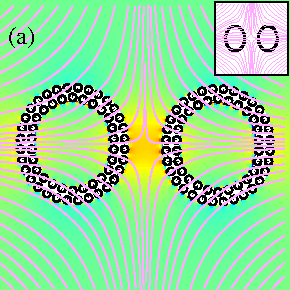
\includegraphics[height=2.in]{N116_ext_0.pdf}
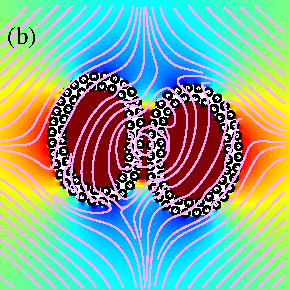
\includegraphics[height=2.in]{N116_ext_2500.pdf}\\
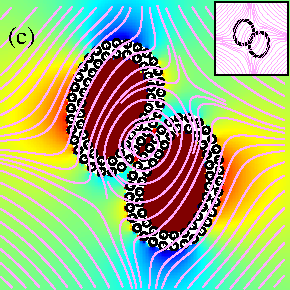
\includegraphics[height=2.in]{N116_ext_5000.pdf}
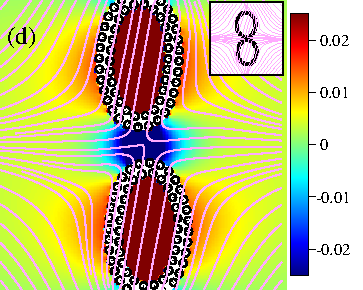
\includegraphics[height=2.in]{N116_ext_7500.pdf}
  \caption{Two vesicles under an extensional flow where the dimensioneless shear rate is $\dot\gamma=0.005$; The initial configuration is shown in panel (a). The background color indicates the magnitude of fluid pressure. From dark red to dark blue, it represents the the pressure varies from high to low values. The color bar is valid for all panels. Streamlines are plotted in purple.
  }
    \label{figure8}
\end{figure}


%\begin{figure}
%\centering
%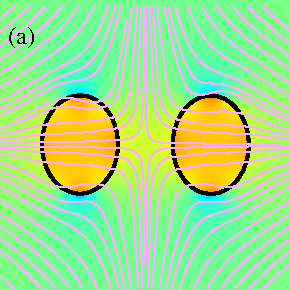
\includegraphics[height=1.2in]{N116_cont_a.pdf}
%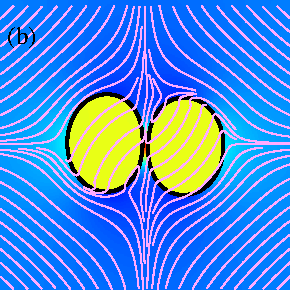
\includegraphics[height=1.2in]{N116_cont_b.pdf}
%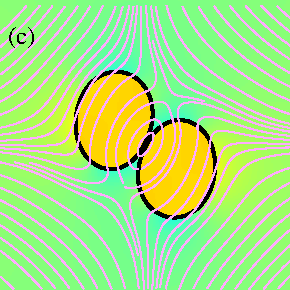
\includegraphics[height=1.2in]{N116_cont_c.pdf}
%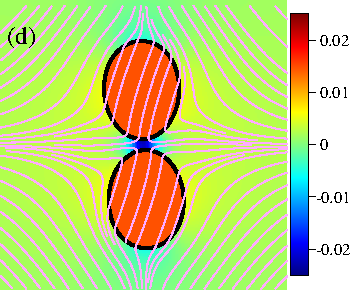
\includegraphics[height=1.2in]{N116_cont_d.pdf}
%  \caption{Two vesicles under an extensional flow where the dimensioneless shear rate is $\dot\gamma=0.005$; Continuum modeling.....
%  }
%    \label{figure8}
%\end{figure}



%\begin{figure}
%\centering
%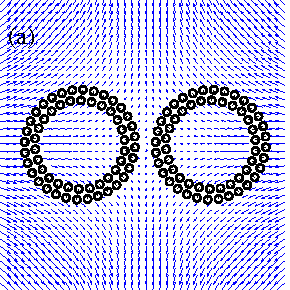
\includegraphics[width=0.24\textwidth]{N116_ext_vel_0.pdf}
%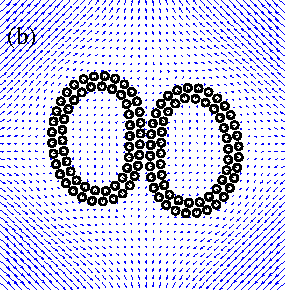
\includegraphics[width=0.24\textwidth]{N116_ext_vel_2500.pdf}
%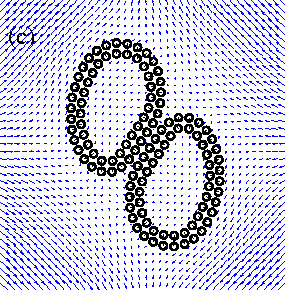
\includegraphics[width=0.24\textwidth]{N116_ext_vel_5000.pdf}
%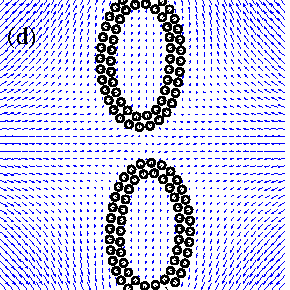
\includegraphics[width=0.24\textwidth]{N116_ext_vel_7500.pdf}
%  \caption{(a)-(d) The background arrows indicate the fluid velocities. }
%    \label{figure6}
%\end{figure}

\subsubsection{Extensional Flow}

Figures~\ref{figure8} show the numerical results of simulations when two vesicles are in an extensional flow. Starting from the initial configuration (shown in panel (a)), panels (b)-(d) show the transitions of two vesicles moving under an extensional flow. The extensional flow is stretching along the $y$ direction and squeezing in $x$ direction with shear rate $\dot\gamma=0.005$. Since two bilayers are close enough
from the beginning of the run, two vesicles are first pushed toward each other then separate along the streamline. The short range repulsion plays an important role to avoid structure collisions and 
this result can be compared with some findings in continuum modeling simulations.
The pressure plots in Figure~\ref{figure8} provide a realistic result where the pressure is much higher in the gap between two nearby vesicles.

%may need to add more here


\begin{figure}
\centering
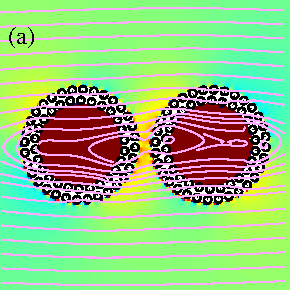
\includegraphics[height=1.2in]{N116_shear_0.pdf}
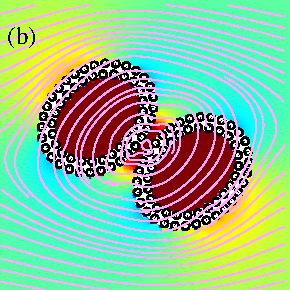
\includegraphics[height=1.2in]{N116_shear_3000.pdf}
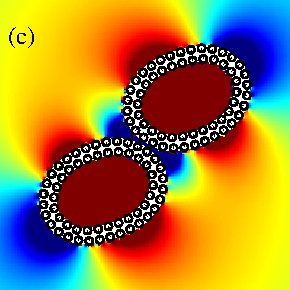
\includegraphics[height=1.2in]{N116_shear_6000.pdf}
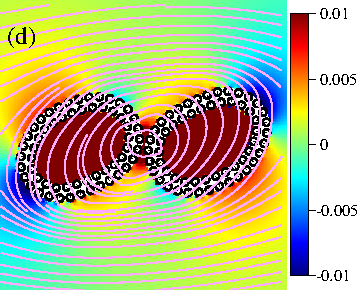
\includegraphics[height=1.2in]{N116_shear_9000.pdf}\\
  \caption{Two vesicles under a shear flow where the dimensioneless shear rate is $\dot\gamma=0.005$; The initial configuration is shown in panel (a). The background color indicates the magnitude of fluid pressure. From dark red to dark blue, it represents the the pressure varies from high to low values. The color bar is valid for all panels. Streamlines are plotted in purple.
  }
    \label{figure9}
\end{figure}



%\begin{figure}
%\centering
%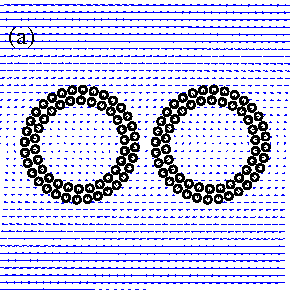
\includegraphics[width=0.24\textwidth]{N116_shear_vel_0.pdf}
%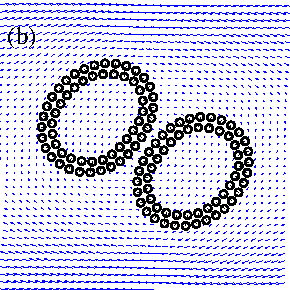
\includegraphics[width=0.24\textwidth]{N116_shear_vel_3000.pdf}
%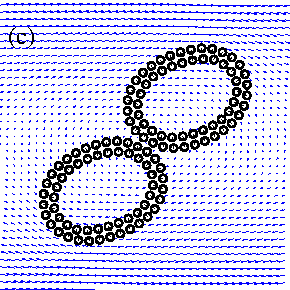
\includegraphics[width=0.24\textwidth]{N116_shear_vel_6000.pdf}
%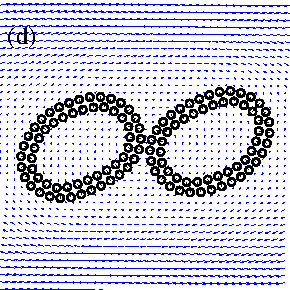
\includegraphics[width=0.24\textwidth]{N116_shear_vel_9000.pdf}
%  \caption{(a)-(d) The background arrows indicate the fluid velocities. }
%    \label{figure8}
%\end{figure}


\subsubsection{Shear Flow}
Two vesicles in a shear flow is resented in Figures~\ref{figure9} where centers of mass are placed on the same horizontal level. With the same starting state as one in the extensional flow, panels (b)-(d) in Figure~\ref{figure8} are the observed phenomena when two vesicles are in a shear flow where the flow is given by $\dot x = \dot\gamma y$. 
An interesting event occurs in the simulation that a rotational behavior with an adhesive effect can be observed and tuned. In other words, the the adhesive behavior will be absent when two vesicles are centered 
at a different level and are well separated in $y$-direction.



\section{\label{conclusion}Conclusion}


\begin{acknowledgments}
%We would like to acknowledge 
\end{acknowledgments}

\appendix

\section{Appendices}
The stress ${\bf T}$ contains the gradient of the double layer potential. This 
introduces an inherent difficulty in evaluating stress on the boundary.
To overcome the difficulty of evaluation on $\Sigma_p$, for instance, we decompose $u$ into singular and nonsingular parts:
\begin{equation}
u = u_p + v_p
\end{equation}
where  
\begin{equation}
u_p(x) = \int_{\Sigma_p} \frac{\partial G(x,y)}{\partial \nu} \eta(y) \,\dif S(y).
\end{equation}
It turns out that the contribution to the force and torque coming from the singular
part vanishes. In particular, we will prove the identity
\begin{equation}
\label{eq:recipforcetorque}
F_p + iG_p= \int_{\Sigma_p} \gamma ({\bf I}+i{\bf X})J_{p} \,\dif S
\end{equation}
where
 \begin{equation}
\label{eq:jumpstress1}
J_{p} = 2\rho^{-1} \eta  v_p \nu 
+ 2\rho \nabla \eta \cdot \tau_i(\nabla v_p \cdot \tau_i \nu -  \nabla v_p \cdot \nu \tau_i).
\end{equation}
Here $\nu$ is the unit normal, $\{\tau_i\}_{i=1}^2$ are orthonormal tangent vectors,
and ${\bf X}$ is the skew symmetric matrix with axial vector $x$, i.e.
\[X_{ij} = \varepsilon_{ikj}x_k,\quad {\bf X}v = x\times v\]
where $\boldsymbol{\varepsilon}$ is the third-order alternating tensor.
We employ the Einstein summation convention and use complex vectors to streamline the presentation, $i^2 = -1$.

The benefit of using \eqref{eq:recipforcetorque} is that the integrand  is nonsingular.
The density function $\eta$ has the same smoothness as the boundary data
and $v_p$ is real-analytic in a neighborhood of $\Sigma_p$.

To prove \eqref{eq:recipforcetorque}, write
\begin{align*}
  {\bf T}
  &=
  \sigma[u_p,u_p]
  +(\sigma[u_p,v_p]
  +\sigma[v_p,u_p])
  +\sigma[v_p,v_p] \\
  &= {\bf T}_1 + {\bf T}_2 + {\bf T}_3
\end{align*}
where
\[
\sigma[u,v]
= \rho^{-1} uv {\bf I} + \rho \nabla u \cdot \nabla v {\bf I} - 2 \rho \nabla u \otimes \nabla v.
\]
\begin{lemma}
  \label{eq:stress_div_lemma}
  \begin{equation}
    \label{eq:decompdivfree}
    \nabla \cdot {\bf T}_j = 0, \quad
    \nabla \cdot (x \times {\bf T}_j) = 0,\quad j = 1, 2, 3.
  \end{equation}
\end{lemma}
\begin{proof}
  Observe that
  \begin{align*}
    (\nabla \cdot {\bf T})_j &=
    \nabla_k   T_{jk} \\
    &= \rho^{-1} 2u \nabla_j u + \rho(2\nabla_{kl}^2 u \nabla_l u  - 2 \nabla_{kj}^2 u \nabla_k u
    - 2 \nabla_j u \nabla_{kk}^2 u )\\
    &=2\rho^{-1}(-\rho^2 \Delta u + u)\nabla_k u .
  \end{align*}
  However, $-\rho^2 \Delta u + u = 0$ and so we get $\nabla \cdot {\bf T} = 0.$
  Furthermore,
  \begin{align*}
    (\nabla \cdot (x\times {\bf T} ))_j
    &= (\nabla \cdot ({\bf X} {\bf T} ))_j
    = \nabla_k (X_{jl} T_{lk})
    = \nabla_k (\epsilon_{jml}x_m T_{lk})\\
    &= \varepsilon_{jml} T_{lm} + \varepsilon_{jml}x_m \nabla_k T_{lk}\\
    &= (\boldsymbol{\varepsilon}:{\bf T} + {\bf x} \times \nabla \cdot {\bf T})_j.
  \end{align*}
  Since ${\bf T}$ is symmetric $\boldsymbol{\varepsilon}:{\bf T} = {\bf 0}$, and we get
  $\nabla \cdot (x \times {\bf T}) = 0$ as well.

  The functions $u_p$ and $v_p$ also solve the equation $-\rho^2 \Delta u + u = 0$.  Thus
  \eqref{eq:decompdivfree} holds for $j = 1, 3$. Finally,
  \eqref{eq:decompdivfree} holds for $j = 2$ because
  ${\bf T}_2 = {\bf T} - {\bf T}_1 - {\bf T}_3$.
\end{proof}


Using Lemma \ref{eq:stress_div_lemma}, we will establish that
\begin{equation}
  \label{eq:prejump}
  F_p + i G_p = \gamma \int_{\Sigma_p}  ({\bf U}_2\nu)^+ - ({\bf U}_2\nu)^-\,\dif S
\end{equation}
where ${\bf U}_j = ({\bf I} + i {\bf X}){\bf T}_j$ for $j = 1, 2, 3.$
The stress ${\bf U}_2$ has a jump discontinuity at $\Sigma_p.$
The plus and minus superscripts denote
the limit taken along points in $U_p^c$ and along points in $U_p$
respectively.
${\bf U}_1$ and ${\bf U}_3$ are real-analytic in a neighborhood of $\overline{U_p}$
and have no jump-discontinuity at $\Sigma_p$.
To derive \eqref{eq:prejump}, we expand
\begin{align*}
  F_p + i G_p
  &= \gamma \int_{\Sigma_p} {\bf T} \nu + ix \times {\bf T} \nu \,\dif S \\
  &= \gamma \int_{\Sigma_p}  {\bf U}_1\nu  + ({\bf U}_2\nu)^+ + {\bf U}_3\nu\,\dif S
\end{align*}
The function $u_p$ is real-analytic and
$\nabla \cdot {\bf U}_1 = 0$ throughout $\mathbb{R}^n \setminus U_p$.
By the divergence theorem, we get
\begin{equation*}
  \int_{\Sigma_p}  {\bf U}_1 \nu\,\dif S
  = \int_{\mathbb{R}^n \setminus U_p} \nabla \cdot {\bf U}_1 \,dx = 0.
\end{equation*}
Next, $v_p$ is real-analytic and
$\nabla \cdot {\bf U}_3 = 0$ in $U_p$. Therefore
\begin{equation*}
  \int_{\Sigma_p}  {\bf U}_3 \nu\,\dif S
  = -\int_{U_p} \nabla \cdot {\bf U}_3 \,dx = 0.
\end{equation*}
Finally, $\nabla \cdot {\bf U}_2= 0$ in $U_p$. This gives
\[
0 = -\int_{U_p} \nabla \cdot {\bf U}_2 \,dx = \int_{\Sigma_p}  ({\bf U}_2 \nu)^-\,\dif S.
\]
Combining the last four equations give \eqref{eq:prejump}.

\begin{proof}[Proof of \eqref{eq:recipforcetorque}]
  The main ingredients of the proof are the jump relations
  for $u_p$. For $x_0 \in \Sigma_p$,
  \begin{enumerate}
  \item $ \lim_{x \to x_0^\pm } u_p(x) = \pm\frac{1}{2}\eta(x_0) + (D\eta)(x_0)$
  \item $ \lim_{x \to x_0^+ } (\nabla u_p \cdot \nu) (x) = \lim_{x \to x_0^-} (\nabla u \cdot \nu)(x)$
  \end{enumerate}
  Furthermore,
  combining (i) and (ii) gives
  \begin{align*}
    \nabla u_p^+ - \nabla u_p^-
    &= \nabla (u_p^+ - u_p^-) \cdot t_i t_i +  (\nabla  u_p^+\cdot \nu  - \nabla u_p^- \cdot \nu) \nu\\
    &= \nabla \eta \cdot \tau_i \tau_i
  \end{align*}
  where $\{\tau_i\}_{i=1}^n$ are an orthonormal tangent vectors.
  We can use these relationships to derive an expression for the jump in
  normal stress.
  \begin{align*}
    &({\bf T}_2\nu)^+ - ({\bf T}_2\nu)^-
    \\
    &= 2\rho^{-1} u_p^+v_p \nu + 2\rho \nabla u_p^+ \cdot \nabla v_p \nu
    - 2 \rho \nabla u_p^+  \nabla v_p \cdot \nu
    - 2 \rho \nabla v_p  \nabla u_p^+ \cdot \nu\\
    &-2\rho^{-1} u_p^-v_p \nu - 2\rho \nabla u_p^- \cdot \nabla v_p \nu
    + 2 \rho \nabla u_p^-  \nabla v_p \cdot \nu
    + 2 \rho \nabla v_p  \nabla u_p^- \cdot \nu\\
    &= 2\rho^{-1} \eta v_p \nu + 2\rho \nabla \eta \cdot \tau_i \tau_i \cdot \nabla v_p \nu
    - 2\rho \nabla \eta \cdot \tau_i \tau_i \nabla v_p \cdot \nu + 0\\
    &= J_p.
  \end{align*}

  Applying the above relations to the integrand of \eqref{eq:prejump} yields
  \[
  ({\bf U}_2\nu)^+ - ({\bf U}_2\nu)^-
  =
  ({\bf I} + i {\bf X})(({\bf T}_2\nu)^+ - ({\bf T}_2\nu)^-)
  = ({\bf I} + i {\bf X})J_p
  \]
  This completes the proof of \eqref{eq:recipforcetorque}.
\end{proof}

%\bibliographystyle{jfm}
\bibliography{reference}% Produces the bibliography via BibTeX.





%\bibliographystyle{jfm}
%\bibliography{jfm}
%Use of the above commands will create a bibliography using the .bib file. Shown below is a bibliography built from individual items.


%\bibliography{jfm2esam}

%\begin{thebibliography}{99}
%
%\expandafter\ifx\csname natexlab\endcsname\relax
%\def\natexlab#1{#1}\fi
%\expandafter\ifx\csname selectlanguage\endcsname\relax
%\def\selectlanguage#1{\relax}\fi
%
%\bibitem[Batchelor (1971)]{Batchelor59}
%{\sc Batchelor, G.K.} 1971 {Small-scale variation of convected quantities like temperature in turbulent fluid part1, general discussion and the case of small conductivity}, {\it J. Fluid Mech.}, {\bf 5}, pp. 3-113-133.
%
%\bibitem [Bouguet (2008)]{Bouguet01}
%{\sc Bouguet, J.-Y} 2008 Camera Calibration Toolbox for Matlab {\url{http://www.vision.caltech.edu/bouguetj/calib_doc/}}.
%
% \bibitem[Briukhanovetal et al (1967)] {Briukhanovetal1967}
%{\sc Briukhanov, A. V.,   Grigorian, S. S., Miagkov,  S. M., Plam, M. Y.,   I. E. Shurova, I. E.,   Eglit, M. E. and Yakimov, Y. L.} 1967
%{On some new approaches to the dynamics of snow avalanches},
%{\it Physics of Snow and Ice,  Proceedings of the International Conference on Low Temperature Science}
%{Vol 1} pp. 1221--1241 {Institute of Low Temperature Science, Hokkaido University, Sapporo, Hokkaido, Japan}.
%
%\bibitem[Brownell (2004)]{Brownell04}
% {\sc Brownell,  C.J.  and Su,  L.K.} 2004  {Planar measurements of differential diffusion in turbulent jets}, {\it AIAA Paper},  pp. 2004-2335.
%
%\bibitem[Brownell and Su (2007)] {Brownell07}
%  {\sc Brownell, C.J. and  Su, L.K.} 2007 {Scale relations and spatial spectra in a differentially diffusing jet}, {\it AIAA Paper}, pp 2007-1314.
%
%\bibitem [Dennis (1985)] {Dennis85}
% {\sc  Dennis, S.C.R.} 1985 {Compact explicit finite difference approximations to the Navier--Stokes equation},  { In \it Ninth Intl Conf. on Numerical Methods in Fluid Dynamics},  {ed Soubbaramayer and J.P. Boujot},  {Vol 218}, {\it Lecture Notes in Physics}, pp. 23-51. Springer.
%
%\bibitem [Edwards et al. (2017)]{EdwardsVirouletKokelaarGray2017}
%{\sc Edwards, A. N., Viroulet, S., Kokelaar, B. P. and Gray, J. M. N. T.} 2017 Formation of levees, troughs and elevated channels by avalanches on erodible slopes {\it J. Fluid Mech.}, {\bf 823}, pp. 278-315.
%
%\bibitem[Hwang et al (1970)] {Hwang70}
% {\sc Hwang,  L.-S.  and  Tuck, E.O.} 1970 On the oscillations of harbours of arbitrary shape {\it J.~Fluid Mech.}, {\bf42}, pp 447-464.
%
%\bibitem[Josep and Saut (1990)] {JosephSaut1990}
% {\sc Joseph, Daniel D. and Saut, Jean Claude} 1990 Short-wave instabilities and ill-posed initial-value problems {\it Theoretical and Computational Fluid Dynamics}, {\bf 1},  pp.191--227,  {\url{http://dx.doi.org/10.1007/BF00418002}}.
%
%\bibitem[Worster (1992)] {Worster92}
%{ \sc  Worster, M.G.} 1992 The dynamics of mushy layers {\it Interactive dynamics of convection and solidification},
%{(ed. S.H. Davis and H.E. Huppert and W. Muller and M.G. Worster)}, pp. 113--138 {Kluwer}.
%
%\bibitem[Koch(1983)] {Koch83}
%{\sc Koch, W.} 1983 Resonant acoustic frequencies of flat plate cascades {\it J.~Sound Vib.}, {\bf 88}, pp. 233-242.
%
%\bibitem[Lee(1971)] {Lee71}
%{\sc Lee,  J.-J.}  1971 Wave-induced oscillations in harbours of arbitrary geometry {\it J.~Fluid Mech.}, {\bf 45}, pp. 375-394.
%
%\bibitem[Linton and  Evans (1992)] {Linton92}
% {\sc  Linton, C.M. and  Evans, D.V.} 1992 The radiation and scattering of surface waves by a vertical circular cylinder in a channel {\it Phil.\ Trans.\ R. Soc.\ Lond.}, {\bf 338}, pp. 325-357.
%
%\bibitem [Martin(1980] {Martin80}
% {\sc  Martin, P.A.} 1980 On the null-field equations for the exterior problems of acoustics {\it Q.~J. Mech.\ Appl.\ Maths},{\bf 33}, pp. 385--396.
%
%\bibitem [Rogallo(1981)] {Rogallo81}
% {\sc Rogallo,  R.S.} 1981 Numerical experiments in homogeneous turbulence  { {\it Tech. Rep.} 81835}  {NASA Tech.\ Mem}.
%
%\bibitem[Ursell(1950)] {Ursell50}
%{\sc  Ursell, F.} 1950 Surface waves on deep water in the presence of a submerged cylinder i {\it Proc.\ Camb.\ Phil.\ Soc.}, {\bf 46}, pp.141--152.
%
%\bibitem[Wijngaarden (1968)]{Wijngaarden68}
%{\sc van Wijngaarden, L.} 1968 On the oscillations Near and at resonance in open pipes {\it J.~Engng Maths},{\bf 2}, pp. 225--240.
%
%\bibitem[Miller (1991)]{Miller91}
%{ \sc  Miller, P.L.} 1991 Mixing in high Schmidt number turbulent jets {school {PhD thesis}} {California Institute of Technology}.
%
%\end{thebibliography}

%% End of file `jfm2esam.bib'.

\end{document}
